\chapter{Our Approach}
\label{chap:ourapp}


In this chapter, we propose a novel approach to evaluate $k$GTP queries. In a $k$GTP query, the group provides the source and destination locations of the group members, $k$, and the required categories of POIs and the query returns $k$ sets of POIs as answer. Road networks are enormous in size with numerous POIs and the operation on all POIs brings huge processing overhead. The underlying idea of our approach is to refine the search space to reduce the number of POIs to be considered. The steps of our solution are as summarized as follows:


\vspace*{5pt}
\textbf{Step 1: } We develop a heuristic technique to retrieve an initial candidate answer set that includes one POI from each category. Then we compute the aggregate distance of the retrieved POIs with respect to the source-destination pairs of the group members.

\vspace*{5pt}
\textbf{Step 2: } Based on the retrieved candidate answer set in the previous step, we refine the search region using elliptical properties. Any data point outside the refined search region cannot minimize the aggregate travel distance.

\vspace*{5pt}
\textbf{Step 3: } This step executes a range query to find all POIs included in the refined region. From the retrieved POIs, our approach finds the actual POIs that provide the minimum aggregate travel distance.

\vspace*{8pt}
In Sections~\ref{sec:step1},~\ref{sec:step2}, and~\ref{sec:step3}, we discuss detail of these three steps. Section~\ref{alg1} shows our algorithms and presents detail discussion. In Section~\ref{flxQ}, we propose our algorithm in a way that can solve flexible $k$GTP queries. 




\section{Selection of Initial POIs}
\label{sec:step1}
In this section, we present a heuristic to retrieve an initial answer set that includes one POI from every requested category. Our heuristic is based on the intuition that the selection of a path for one user affects all others in the group. We first show how our heuristic works for a $k$GTP query, when the visiting order of POIs is fixed.

Our developed heuristic first computes geometric centroid, $c_s$ and $c_d$, with respect to the set of source and destination locations of the group members, respectively. From \textit{c$_{s}$} to \textit{c$_{d}$}, we apply Nearest Neighbor (NN) search greedily for the next POI from the ordered categories. This initial answer set $P$ contains a POI from each required category. Without loss of generality, Figure~\ref{fig:centroid} shows an example, where a GTP query needs to be evaluated from 3 categories of POIs $C_1$, $C_2$, and $C_3$, $k=1$ and for source and destination sets, $\{s_1, s_2, s_3\}$ and $\{d_1, d_2, d_3\}$, respectively. Our heuristic first finds nearest neighbor $p_1$ of $c_s$ from $C_1$, then the nearest neighbor $p_2$ of $p_1$ from $C_2$, and finally, the nearest neighbor $p_3$ of $p_2$ from $C_3$.

\vspace*{12pt}
\begin{figure}[!htbp]
\centering
\includegraphics[width=0.6\columnwidth]{figures/soln1/centroid.pdf}
\caption{Centroid method}
\label{fig:centroid}
\end{figure}
\vspace*{10pt}
For each user $u_i$ ($i=1,2,..., n$), our approach computes the trip distance $T_i$ from $s_i$ to $d_i$ via $p_1$, $p_2$, \dots $p_m$. Then we apply the aggregate function $f$ to determine the aggregate trip distance as $d_{best}$ for the initial answer set, $P_{dum}$. To remind the reader, for \textsc{sum}, the aggregate distance is $\sum_{i=1}^{n} T_i$ and for \textsc{max}, the aggregate distance is $\max_{i=1}^{n} T_i$.

\vspace*{5pt}
For $k>1$, our heuristic retrieves $k$ nearest neighbors from $C_m$ with respect to $p_{m-1}^1$ as $p_m^1, p_m^2, \dots p_m^k$. Our approach computes aggregate travel distances for $k$ sets of POIs $\{p_1, p_2,..., p_m^1\}$, $\{p_1, p_2,..., p_m^2\}$, \dots, $\{p_1, p_2,..., p_m^k\}$ and initializes $d_{best}^k$ with the maximum of these aggregate distances.

In a flexible $kGTP$ query, the order of visiting POI category is not fixed. The group only mentions the required POI categories and is happy to visit the POIs in any order that minimizes the aggregate travel distance. In a flexible $kGTP$ query, our approach randomly selects an order of visiting POI categories and then apply the same heuristic for the ordered $k$GTP query discussed above to retrieve the initial answer set $P_{dum}$ for that order. After retrieving the initial POIs, our approach computes aggregate trip distances for all POI sets considering all possible orders and initializes $d_{best}^k$ with the $k^{th}$ minimum of these aggregate distances. For example,  if the $P=\{p_1,p_2,p_3\}$ then the possible sets are $\{p_1,p_2,p_3\}$, $\{p_1,p_3,p_2\}$, $\{p_2,p_1,p_3\}$,$\{p_2,p_3,p_1\}$,$\{p_3,p_1,p_2\}$, and $\{p_3,p_2,p_1\}$.

\section{Refinement of Search Region}
\label{sec:step2}

We use the minimum distance $d_{best}^k$ from step 1 to reduce the search space from the \textit{whole search region} to a \textit{refined search region} for both ordered and flexible $k$GTP queries. The whole road networks with numerous data points of various categories is the \textit{whole search region}. The search for the solution in this whole region is infeasible. We refine the search space using $d_{best}^k$ as follows:

We consider $n$ ellipses $E_1,E_2,...,E_n$  for each user $u_1,u_2,...,u_n$. Ellipse $E_i$ has foci at $s_i$ and $d_i$, and length of the major axis equal to $d_{best}^k$. Let, $E_{int}$ be the intersection region of the ellipses, i.e., $E_{int} = \cap_{i=1}^n E_i$. We confine the search only within $E_{int}$.


\begin{figure}[!htbp]
\centering
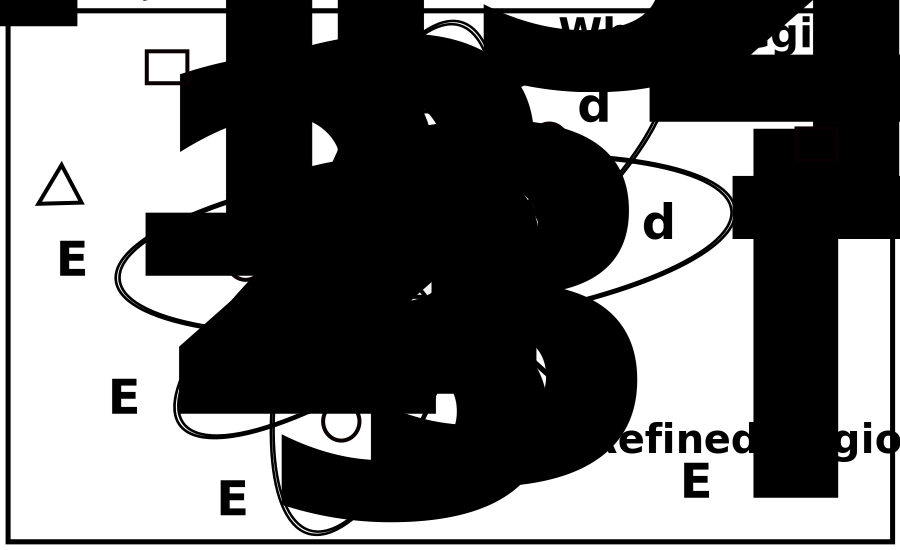
\includegraphics[width=0.6\columnwidth]{figures/soln1/proof.pdf}
\caption{Refined search region}
\label{fig:proof}
\end{figure}
The following lemma and theorem show that the optimal answer resides within $E_{int}$.\\

\hspace{-3ex}\textsc{lemma} 1: \textit{$E_{int} \neq \emptyset $}

\begin{proof}
Let, $p$ be a data point in the $k^{th}$ optimal solution found so far. For any arbitrary user $u_l$ (where $1 \le l \le n),  d(s_l,p)+d(p,d_l)<T_l$ where $T_l$ is the trip distance of $u_l$ in the $k^{th}$ optimal solution. In case of sum aggregate function, $T_l < \sum_{i=1}^n T_i \le d_{best}^k$, since $d_{best}^k$ is the value of current best solution for \textsc{sum} aggregate function. So, we find that $d(s_l,p) + d(p,d_l) < d_{best}^k$. This implies that point $p$ resides inside the ellipse $E_l$ (For any point inside an ellipse, the summation of distances from the point to the two foci is less than the major axis length). Since, $u_l$ was chosen arbitrarily, point $p$ must reside inside all ellipses $E_1,E_2,...,E_n$. This means the intersection region $E_{int}$ is non-empty.
\end{proof}



\begin{theorem}
The intersection of the regions $E_{int}$ bounded by ellipses $E_1,E_2$, ..., $E_n$ contains all the data points that constitute optimal solutions.
\end{theorem}

\begin{proof}
(By contradiction). Let, $p$ be a data point outside the region $E_{int}$ and is a part of $j^{th}$ optimal solution where $1 \le j \le k$. Since, $p$ is outside $E_{int}$, it is outside of at least one of the ellipses $E_1,E_2,...,E_n$. Let, $E_l$ be such an ellipse that do not contain the point $p$ where $1 \le l \le n$.

Since, user $u_l$ passes through the data point $p$, the trip distance $T_l$ in the $j^{th}$ optimal solution cannot be less than $d(s_l,p)+d(p,d_l)$, i.e., $T_l \geq d(s_l,p)+d(p,d_l)$. According to the properties of ellipses, for any point outside of an ellipse, the summation of the distances from the point to the two foci is greater than its major axis length. Hence, for ellipse $E_l,  d(s_l,p)+d(p,d_l )>d_{best}^k$. But, $T_l \geq d(s_l,p)+d(p,d_l)$. So, $T_l>d_{best}^k$.

Now, consider \textsc{sum} aggregate function first. Then, total group distance for $j^{th}$ solution will be greater than $d_{best}^k$ as shown by
$\sum_{i=1}^n T_i > T_l > d_{best}^k.$

But, $d_{best}^k$ is the current best value for $k^{th}$ optimal solution. So, $j^{th}$ solution value cannot be greater than $d_{best}^k$. (Contradiction)

In case of \textsc{max} aggregate function, the maximum distance traveled by any user will also be greater than $d_{best}^k : max_{i=1}^n T_i > T_l > d_{best}^k $, however, $d_{best}^k$ is the current best value of $k^{th}$ solution. (Contradiction).
\end{proof}

\vspace*{6pt}
\section{Optimal Answer Computation}
\label{sec:step3}

In this step, our approach executes a range query on the POIs in the candidate answer set \textit{CA} which resides inside the intersection of ellipses, $E_{int}$. The application of brute force technique to extract the solution increases the complexity with the increase of categories and users. We use $d_{best}^k$ as current threshold for the aggregate trip distance and further prune the POIs, which makes the partial aggregate distance greater than $d_{best}^k$.

Specifically, we traverse starting from the source set $S$, pass through all categorized POIs in order and react at destination set $D$. If at any stage the cumulative distance greater than $d_{best}^k$, the traversal stops along the path. Each time a smaller cumulative distance appears by the traversal from source \textit{s$_{i}$} to corresponding destination \textit{d$_{i}$} through the ordered categorized POIs, we update $d_{best}^k$. Note that for flexible $k$GTP queries, we have to repeat the traversal of candidate POIs in all possible orders.

In Figure~\ref{fig:range}, let the predefined value for $d_{best}^k$ is 19. Two categories $C_1$ and $C_2$ exist such that POIs \{$p_1^{'}, p_1^{''}, p_1^{'''}\} \in C_1$ and \{$p_2^{'}, p_2^{''}, p_2^{'''}\} \in C_2$. The traversal along path $s_1 - p_1^{'} - p_2^{'} - d_1$ is completely forsaken after visiting node $p_2^{'}$. Because at that node, the cumulative distance along that path is 20 which exceeds the range value 19. For another case, along the path $s_1 - p_1^{''} - p_2^{''} - d_1$, the cumulative distance becomes 15 at the destination point. This value is smaller than the predefined range $d_{best}^k$. So 15 becomes the new range value of $d_{best}^k$.

\vspace*{12pt}
\begin{figure}[!htbp]
\centering
\includegraphics[width=0.6\columnwidth]{figures/soln1/range.pdf}
\caption{Optimal answer selection}
\label{fig:range}
\end{figure}

\vspace*{12pt}
\section{Algorithms}
\label{alg1}

Algorithm 1 shows the details steps for processing an ordered $k$GTP queries. The POIs are indexed using an $R$-tree in the database. The source location set \textit{S}, the destination set \textit{D}, the category set \textit{C}, the aggregate function to be minimized \textit{f} and $k$ are the inputs. The output \textit{A} is $k$ sets of POIs that have $k$ smallest trip distances.

Algorithm 1 starts with initializing the variables $A$, $dist$ and $d_{best}^k$. Then the algorithm applies our heuristic to retrieve the initial POIs from required categories (Lines 4--11). The algorithm uses function $FindCentroid$ to compute geometric centroid, $c_s$ and $c_d$, with respect to the source and destination set, respectively. From $c_s$, the algorithm finds the greedy nearest neighbor $y$ from category $C_1$ by using the function $FindNN$. The input to $FindNN$ are $c_s$ (from which the NN will be computed), $C_1$ (from which category the NN will be computed) and $1$ (the number of requested NN). Any existing nearest neighbor algorithm in road networks can be used for this purpose. $P$ stores the the POIs computed using the proposed heuristic.

The function $ElementNum$ returns the number of categories in set $C$. Starting from the first category, $FindNN$ function returns the nearest neighbor of the next category with respect to the POI of the previous category, until the next category is $C_{m-2}$. All these neighbors are stored in $P$. Then the algorithm find $k$ NNs from category $C_m$ with respect to the identified POI $p_{m-1}$.

The algorithm uses the function $CalcBestD$ to compute $k^{th}$ aggregate distance with respect to $f$ and assigns it to the variable $d_{best}^k$. $CalcBestD$ takes $S, D, P, k, f$ as inputs and computes $k$ possible sets from POIs stored in $P$: $\{p_1, p_2,..., p_m^1\}$, $\{p_1, p_2,..., p_m^2\}$, \dots, $\{p_1, p_2,..., p_m^k\}$. $CalcBestD$ computes the aggregate trip distance for each set and returns the maximum one as $k^{th}$ aggregate distance.


\textbf{\textit{CalcBestD}} function is described in Algorithm~\ref{alg:calcd}. It takes in the parameters $S, D, P, k, f$ and produces the value of $d_{best}^k$ as output. To compute trip distances, we apply network distance function $d$ for each user for each values of $k$. For each user, the cases considered are as follows: source to POI of category-1, POI of category-1 to ordered POIs in categories up to category-$(m-2)$, POI of category-$(m-1)$ to $j^{th}$ POI of category-$m$, $j^{th}$ POI of category-$m$ to destination, where $j={1,2, \dots k}$. These are all added to produce total trip distance $T_i$ for each user in Line 11. Then, if the case is for \textsc{sum}, adding the maximum trip distances for each user gives the greedy best distance, shown in Line 15. Otherwise for \textsc{max}, \textsc{max} function in Line 17 gives the maximum value of trip distances for all users and the value is assigned to $d_{best}^k$.


In the second step, the algorithm executes $CandidateSet$, which takes three parameters $S,D,d_{best}^k$ as inputs and returns all POIs in the refined search region as $CA$. More specifically, $CandidateSet$ first computes the individual ellipses, compute the intersection of ellipses and then execute a range query to retrieve the POIs within the intersection of ellipses from the database.

After getting the candidate set $CA$, the algorithm searches for set of POIs $k$ optimal trips have been found. The function $RangeQf$ executes a search for $k$ trips based on $d_{best}^k$. $RangeQf$ maintains the following characteristics: the search towards a path terminates if the cumulative distance found so far exceeds $d_{best}^k$ value. Each time an aggregate trip distance $dist$ is smaller than $d_{best}^k$, $d_{best}^k$ and $A$ are updated.

\begin{algorithm}[!htbp] %previously !htbp
 % \small{}
%  \texttt{}
 \caption{\emph{kGTPQ}}
 \label{alg:gtpq}

Input:  \textit{S, D, C, f, k}

Output: \textit{A}

\begin{algorithmic}[1]
\STATE $A \leftarrow $null, $P \leftarrow $null, $dist \leftarrow $0, $d_{best}^k \leftarrow $0, $i \leftarrow $1, $m \leftarrow 0$
\STATE $c_{s} \leftarrow FindCentroid$($S)$
\STATE $c_{d} \leftarrow FindCentroid$($D)$

\STATE $y \leftarrow FindNN$($c_{s}$,$C_{1}, 1)$
%\STATE $d_{best} \leftarrow $(d($s_{1}$,$c_{s}$)+GreedyDist$(x,y)$)	
\STATE $P \leftarrow P \cup \{y\}$
\STATE $m \leftarrow ElementNum(C)$
\WHILE {$i \le $(m-2)}
	\STATE $x \leftarrow $$y$
	\STATE $y \leftarrow FindNN(x,C_{i+1},1)$
%   	\STATE $d_{best} \leftarrow $($d_{f}+GreedyDist$(x,y))	
	\STATE $ P \leftarrow P \cup \{y\}$
	\STATE $i \leftarrow i$+1
 \ENDWHILE 	
%\STATE $d_{f} \leftarrow $($d_{f}+$d($c_{d}$,$d_1$)+$GreedyDist$(y,$c_{d})$)
\STATE $P \leftarrow P \cup FindNN(p_{m-1},C_{m},k)$
\STATE $d_{best}^k \leftarrow CalcBestD(S,D,P,k,f)$
\STATE $CA \leftarrow CandidateSet(S,D,d_{best}^k)$

\STATE $i \leftarrow $1
\REPEAT
\FOR {every $p_1^{i}$  in   $C_1 \in CA$}

\STATE $dist \leftarrow RangeQf(S,D,CA,f,p_{i}^1,d_{best}^k))$


\IF {$dist<d_{best}^k$}
\STATE $d_{best}^k \leftarrow $dist
\STATE $A \leftarrow A \cup RangeSet(S,D,p_1^i,d_{best}^k)$


\ENDIF
\ENDFOR

\UNTIL All \textit{k} sets are found
 \end{algorithmic}
 \end{algorithm}






\begin{algorithm}[!htbp] %previously !htbp
 % \small{}
%  \texttt{}
 \caption{\emph{CalcBestD}}
 \label{alg:calcd}

Input:  \textit{$S,D,c_s,c_d,P,k,f$} 

Output: \textit{$d_{best}^k$}
 
\begin{algorithmic}[1]
\STATE $d_{best}^k \leftarrow $0, $T \leftarrow null $, $i \leftarrow $1, $j \leftarrow $1, $m \leftarrow 0$, $n \leftarrow $0, $r \leftarrow $1
\STATE $m \leftarrow ElementNum(P)$
\STATE $n \leftarrow ElementNum(S)$

\FOR {$i \le n$}
\IF {($m = $1)}
\STATE $p_{m-1} \leftarrow s_i$ 
\STATE $p_1 \leftarrow s_i$
\ENDIF
\STATE $j \leftarrow 1$ 
\FOR {$j \le k$}
\STATE $T_i^j \leftarrow d(s_i,p_1) + \sum_{r=1}^{m-2} d(p_r,p_{r+1}) + d(p_{m-1},p_{m}^j$) $ + d(p_m^j,d_i) $
\ENDFOR
\ENDFOR
\IF {$f$ denotes \textsc{sum}}

\STATE $d_{best}^k = \sum_{i=1}^{n} (max_{j=1}^k (T_i^j))$
\ELSIF {$f$ denotes \textsc{max}} \STATE $d_{best}^k = max_{i=1,j=1}^{i \le n,j \le k} (T_i^j)$
\ENDIF

 \end{algorithmic}
 \end{algorithm} 


\section{Handling Flexible $k$GTP Queries}
\label{flxQ}
For flexible $k$GTP queries, as we have already mentioned in Sections~\ref{sec:step1} and~\ref{sec:step3}, the algorithms need to determine paths by taking all possible orders of POI categories into consideration while computing distances $d_{best}^k$ and $dist$. For other steps, the algorithm for flexible $k$GTP queries works in the similar way of ordered $k$GTP queries.





















